\section{Pascal VOC2007}

Ovaj skup podataka \citep{pascal-voc-2007} također sadrži slike objekata u svakidašnjem okruženju. Ovdje se nalazi $9963$ slike sa $24 640$ objekata podijeljenih u $20$ kategorija:
\begin{itemize}
	\item \textbf{Person}: person
    \item \textbf{Animal}: bird, cat, cow, dog, horse, sheep
    \item \textbf{Vehicle}: aeroplane, bicycle, boat, bus, car, motorbike, train
    \item \textbf{Indoor}: bottle, chair, dining table, potted plant, sofa, tv/monitor
\end{itemize}
U ovom skupu podataka, slike su označene kao okviri (koordinate okvira).

\begin{figure}[h]
	\centering
	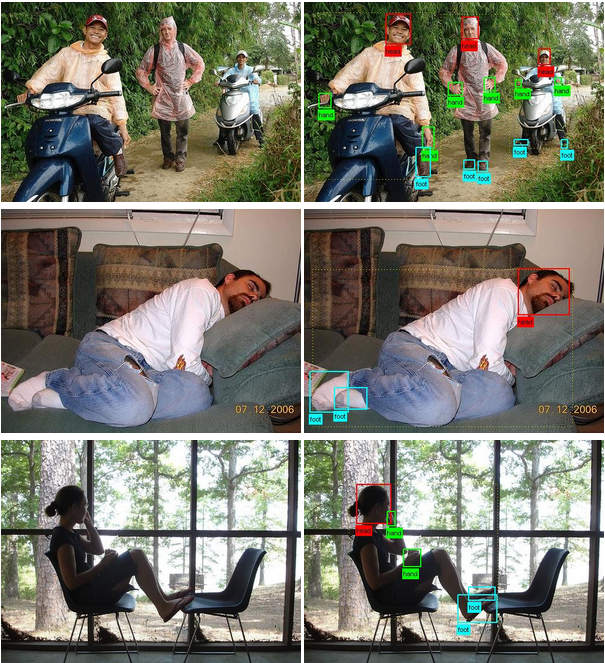
\includegraphics[width=9cm]{/home/luka/Workspaces/diplomski-rad/img/PascalVOC2007.png}
	\caption{Primjeri slika iz skupa Pascal VOC2007, \citep{pascal-voc-2007}}
	\label{img:pascalVOC2007}
\end{figure}

\section{COCO}

COCO (\textit{Common Object in Context}) \citep{coco} je skup podataka nastao 2014. godine. Kako i samo ime nalaže, COCO sadrži preko $330$ tisuća označenih slika sa $1.5$ milijuna označenih objekata u svakidašnjem okruženju i scenama te na taj način tim objektima pridružuje "kontekst". Ovaj skup podataka služi za treniranje algoritama čija je zadaća detekcija i klasifikacija objekata. COCO sadrži objekte podijeljene u $80$ klasa. Na slikama se nalazi više objekata od kojih su svi označeni i segmentirani tako da se na ovom skupu podataka može vršiti i trening mreže za segmentaciju slika. 

\begin{figure}[htp]
	\centering
	\begin{subfigure}[b]{0.4\linewidth}
		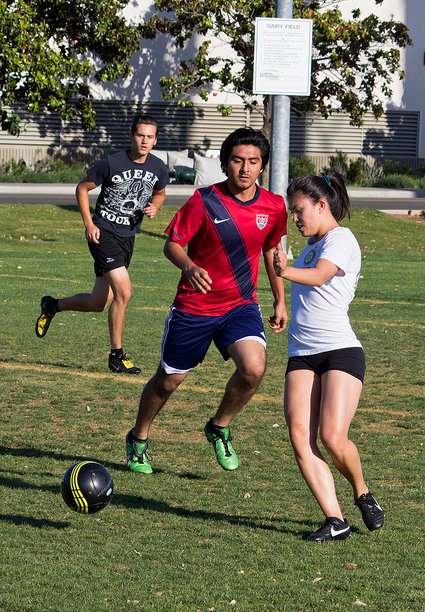
\includegraphics[width=\linewidth]{/home/luka/Workspaces/diplomski-rad/img/COCO1.png}
	\end{subfigure}
	\begin{subfigure}[b]{0.4\linewidth}
		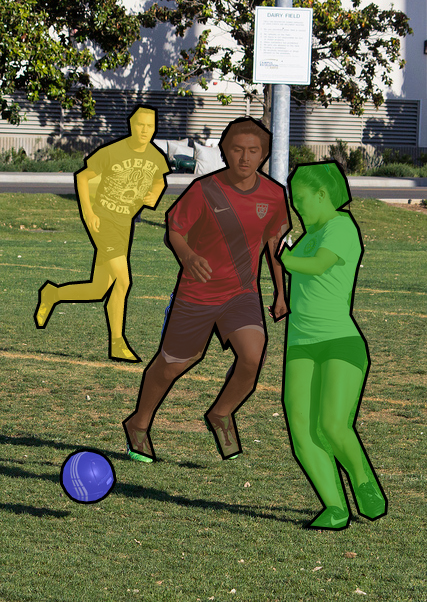
\includegraphics[width=\linewidth]{/home/luka/Workspaces/diplomski-rad/img/COCO11.png}
	\end{subfigure}
	\begin{subfigure}[b]{0.4\linewidth}
		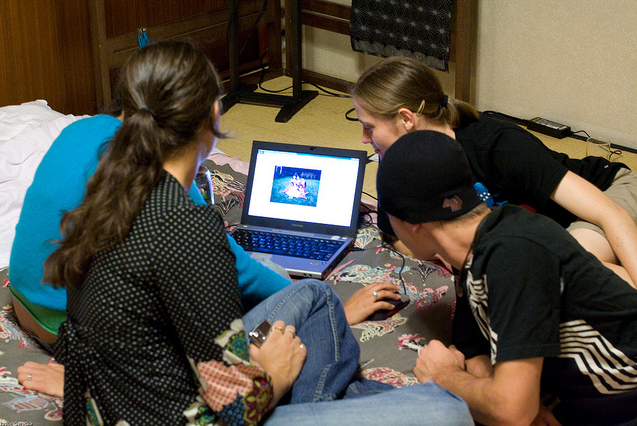
\includegraphics[width=\linewidth]{/home/luka/Workspaces/diplomski-rad/img/COCO2.png}
	\end{subfigure}
	\begin{subfigure}[b]{0.4\linewidth}
		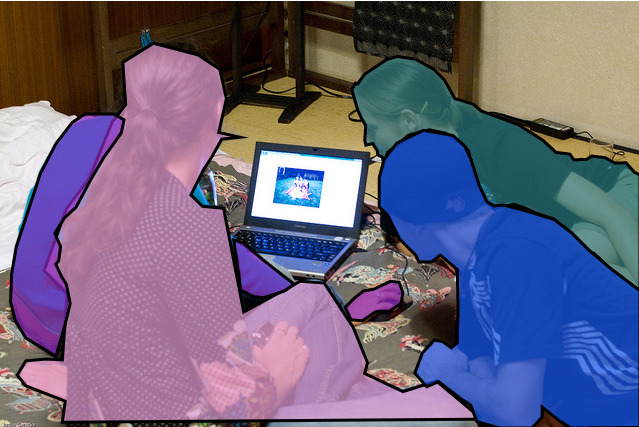
\includegraphics[width=\linewidth]{/home/luka/Workspaces/diplomski-rad/img/COCO22.png}
	\end{subfigure}
	\begin{subfigure}[b]{0.4\linewidth}
		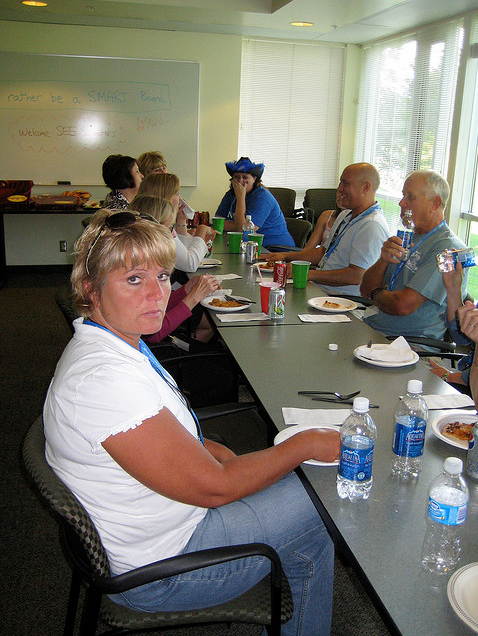
\includegraphics[width=\linewidth]{/home/luka/Workspaces/diplomski-rad/img/COCO3.png}
	\end{subfigure}
	\begin{subfigure}[b]{0.4\linewidth}
		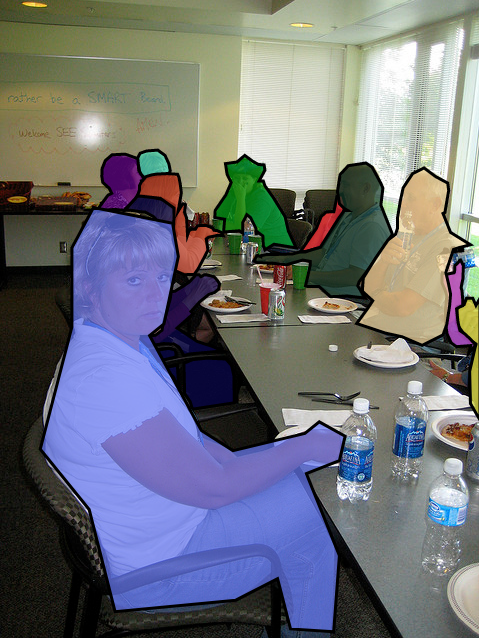
\includegraphics[width=\linewidth]{/home/luka/Workspaces/diplomski-rad/img/COCO33.png}
	\end{subfigure}
	\caption{Primjer slika i oznaka iz COCO skupa podataka, \citep{coco}}
	\label{img:coco-samples}
\end{figure}

\section{Video}

U ovom radu, istraživanje je provedeno na videu 'Esquina Democratica.mp4' preuzetom sa web lokacije: \textit{https://www.videezy.com/people/4966-people-and-commerce-in-a-street-one-point-perspective}. Ovaj video je rezolucije $1920x1080$ te sadrži 30 slika u sekundi videa (30 FPS).


